\documentclass[phdthesis,12pt,final]{wuthesis}

\usepackage{lmodern}


% Remove or comment out the following lines as they're now in wuthesis.tex
% \documentclass[phdthesis,12pt,final]{wuthesis}



\usepackage{ifluatex}
\ifluatex
  \usepackage{fontspec} % international characters
  \usepackage{polyglossia}
  \setmainlanguage[variant=american]{english}
\else % use for pdflatex
  \usepackage[utf8]{inputenc}
  \usepackage[T1]{fontenc}
  \usepackage[american]{babel}
\fi

\usepackage{booktabs}
\usepackage{fancyhdr} % for pagination
\usepackage{microtype} % typographical perfection
\usepackage{csquotes}
\usepackage[vskip=0pt,begintext=\textooquote,endtext=\textcoquote]{quoting}
\SetBlockEnvironment{quoting}

\usepackage[
  backend=biber,
  isbn=false,
  url=false,
  sortcites,
  maxbibnames=8
]{biblatex}

% customzing fonts
\usepackage{titlesec}
\usepackage{tocloft}
\usepackage{anyfontsize}

% Define a consistent font size for title and chapters
\newcommand{\maintitlesize}{\fontsize{16}{20}\selectfont}

% Center and format chapter headings
\titleformat{\chapter}[display]
{\normalfont\maintitlesize\bfseries\centering}
{\chaptertitlename\ \thechapter}{20pt}{\maintitlesize}
\titlespacing*{\chapter}{0pt}{-50pt}{40pt}

% change section headings font size
\titleformat{\section}
{\normalfont\large\bfseries}{\thesection}{1em}{}

% Format List of Tables
\renewcommand{\cfttoctitlefont}{\hfill\maintitlesize\bfseries}
\renewcommand{\cftaftertoctitle}{\hfill}
\renewcommand{\cftlottitlefont}{\hfill\maintitlesize\bfseries}
\renewcommand{\cftafterlottitle}{\hfill}

% Format List of Figures
\renewcommand{\cftloftitlefont}{\hfill\maintitlesize\bfseries}
\renewcommand{\cftafterloftitle}{\hfill}

% Adjust spacing for List of Tables and List of Figures
\setlength{\cftbeforelottitleskip}{-50pt}
\setlength{\cftbeforeloftitleskip}{-50pt}
\setlength{\cftaftertoctitleskip}{40pt}
\setlength{\cftafterlottitleskip}{40pt}
\setlength{\cftafterloftitleskip}{40pt}

% Single-space within entries, double-space between entries
\renewcommand{\cftbeforetabskip}{2em}
\renewcommand{\cftbeforefigskip}{2em}

% general packages
\usepackage{amsmath}
\usepackage{amsfonts}
\usepackage[section]{placeins} % stop floats at sections
\usepackage[inline, shortlabels]{enumitem}
\usepackage{threeparttable}
\usepackage{array}
\usepackage{siunitx}
\usepackage{makecell}
\newcommand{\stretchtable}[1][1.4]{\renewcommand{\arraystretch}{#1}}
\usepackage{mdframed}

% ensure vitaauctoris always starts on a new page
\usepackage{etoolbox}
\pretocmd{\chapter}{\clearpage}{}{}

% use links in document. load last.
\usepackage[hidelinks,linktoc=all]{hyperref}
\usepackage[noabbrev]{cleveref}
\newcommand{\crefrangeconjunction}{--}
\usepackage{caption}

\providecommand{\tightlist}{%
  \setlength{\itemsep}{0pt}\setlength{\parskip}{0pt}}

% for bib
\addbibresource{book.bib}

% style something
\usepackage{fancyvrb}
\usepackage{xcolor}

% Define Shaded and Highlighting environments
\newenvironment{Shaded}{}{}
\newenvironment{Highlighting}{}{}

% Define syntax highlighting commands
\newcommand{\pandocbounded}[1]{#1}

\newcommand{\AttributeTok}[1]{\textcolor[rgb]{0.77,0.63,0.00}{\textbf{#1}}}
\newcommand{\FunctionTok}[1]{\textcolor[rgb]{0.00,0.00,0.75}{#1}}
\newcommand{\NormalTok}[1]{#1}
\newcommand{\ConstantTok}[1]{\textcolor[rgb]{0.53,0.00,0.00}{#1}}
\newcommand{\StringTok}[1]{\textcolor[rgb]{0.31,0.60,0.02}{#1}}
\newcommand{\KeywordTok}[1]{\textcolor[rgb]{0.13,0.29,0.53}{\textbf{#1}}}
\newcommand{\DataTypeTok}[1]{\textcolor[rgb]{0.13,0.29,0.53}{#1}}
\newcommand{\CommentTok}[1]{\textcolor[rgb]{0.56,0.35,0.01}{\textit{#1}}}
\newcommand{\OtherTok}[1]{\textcolor[rgb]{0.56,0.35,0.01}{#1}}
\newcommand{\OperatorTok}[1]{\textcolor[rgb]{0.00,0.00,0.00}{#1}}
\newcommand{\ErrorTok}[1]{\textcolor[rgb]{0.64,0.00,0.00}{\textbf{#1}}}
\newcommand{\WarningTok}[1]{\textcolor[rgb]{0.56,0.35,0.01}{\textbf{\textit{#1}}}}

% Additional syntax highlighting commands for R code
\newcommand{\DecValTok}[1]{\textcolor[rgb]{0.00,0.00,0.81}{#1}}
\newcommand{\BaseNTok}[1]{\textcolor[rgb]{0.00,0.00,0.81}{#1}}
\newcommand{\FloatTok}[1]{\textcolor[rgb]{0.00,0.00,0.81}{#1}}
\newcommand{\CharTok}[1]{\textcolor[rgb]{0.31,0.60,0.02}{#1}}
\newcommand{\SpecialCharTok}[1]{\textcolor[rgb]{0.00,0.00,0.00}{#1}}
\newcommand{\SpecialStringTok}[1]{\textcolor[rgb]{0.31,0.60,0.02}{#1}}
\newcommand{\VerbatimStringTok}[1]{\textcolor[rgb]{0.31,0.60,0.02}{#1}}
\newcommand{\ImportTok}[1]{#1}
\newcommand{\ControlFlowTok}[1]{\textcolor[rgb]{0.00,0.44,0.13}{\textbf{#1}}}
\newcommand{\BuiltInTok}[1]{#1}
\newcommand{\ExtensionTok}[1]{#1}
\newcommand{\PreprocessorTok}[1]{\textcolor[rgb]{0.56,0.35,0.01}{\textit{#1}}}
\newcommand{\DocumentationTok}[1]{\textcolor[rgb]{0.56,0.35,0.01}{\textbf{\textit{#1}}}}
\newcommand{\AnnotationTok}[1]{\textcolor[rgb]{0.56,0.35,0.01}{\textbf{\textit{#1}}}}
\newcommand{\CommentVarTok}[1]{\textcolor[rgb]{0.56,0.35,0.01}{\textbf{\textit{#1}}}}
\newcommand{\VariableTok}[1]{\textcolor[rgb]{0.00,0.00,0.00}{#1}}
\newcommand{\InformationTok}[1]{\textcolor[rgb]{0.56,0.35,0.01}{\textbf{\textit{#1}}}}

%%%%%%%%%%%%%%%%%%%%%%%%%%%%%%%%%%%%%%%%%%%%%%%%%%%%%%%%%%%%%%%%%%%%%%%%%%%%%
%%
%% These commands customize the `wuthesis' package for me
%%
%%%%%%%%%%%%%%%%%%%%%%%%%%%%%%%%%%%%%%%%%%%%%%%%%%%%%%%%%%%%%%%%%%%%%%%%%%%%%

%% Enter your official name
\renewcommand{\thesisauthor}{Montaque Reynolds}
\renewcommand{\thesisauthorlastname}{Reynolds}

%% Enter your previous degrees
%% If you have no previous degrees remember to remove the comma too.
\renewcommand{\thesisauthorpreviousdegrees}{, M.A.}

%% Enter department name
\renewcommand{\thesisdepartment}{Department of Philosophy}
\renewcommand{\thesisfield}{Philosophy}

%% Enter date of graduation
\renewcommand{\thesismonth}{August}
\renewcommand{\thesisyear}{2024}

%% Enter title of thesis
\renewcommand{\thesistitle}{EMOTIONAL DATA AND THE MORAL EXPRESSIONS OF SENTIMENT IN FICTION}

%% Enter the copyright holder ( DEFAULT is \thesisauthor )
%\renewcommand{\thesiscopyrightholder}{\thesisauthor}

%% Enter supervisor name
\renewcommand{\thesissupervisor}{Professor Dan Haybron, Chair\\
Scott Ragland, Co-Chair}
%%
% list in alphabetical order
%%
\renewcommand{\thesiscommittee}{Dan Haybron, Chair\\
Scott Ragland, Co-Chair \\
Scott Gelfand \\
Helen De Cruz}

\renewcommand{\thesisdedication}{Dedicated to my parents.}

\hypersetup{
  pdftitle={\thesistitle},
  pdfauthor={\thesisauthor},
  pdfpagemode=UseOutlines,
  bookmarksnumbered=true,
  bookmarksopen=true,
  bookmarksopenlevel=1
}



\usepackage{amsthm}
\newtheorem{theorem}{Theorem}[chapter]
\newtheorem{lemma}{Lemma}[chapter]
\newtheorem{corollary}{Corollary}[chapter]
\newtheorem{proposition}{Proposition}[chapter]
\newtheorem{conjecture}{Conjecture}[chapter]
\theoremstyle{definition}
\newtheorem{definition}{Definition}[chapter]
\theoremstyle{definition}
\newtheorem{example}{Example}[chapter]
\theoremstyle{definition}
\newtheorem{exercise}{Exercise}[chapter]
\theoremstyle{definition}
\newtheorem{hypothesis}{Hypothesis}[chapter]
\theoremstyle{remark}
\newtheorem*{remark}{Remark}
\newtheorem*{solution}{Solution}
\begin{document}


% Title Page
\begin{titlepage}
\begin{center}
\vspace*{0.5in} % Adjust this value to move the title up or down

{\large\MakeUppercase{Emotional Data and The Moral Expressions of Sentiment in Fiction}\par}

\vspace{1in} % Adjust this space between title and author name

{\large Montaque Reynolds\par}

\vspace{2in} % Adjust this space as needed

A Dissertation Presented to the Graduate Faculty of\\
Saint Louis University in Partial Fulfillment\\
of the Requirements for the Degree of\\
Doctor of Philosophy

\vfill % This will push the year to the bottom of the page

2024

\end{center}
\end{titlepage}

\pagenumbering{roman}
\setcounter{page}{2}

% Copyright Page
\cleardoublepage
\thispagestyle{empty}
\begin{thesiscopyrightpage}
    \vspace*{\fill}
    \begin{center}
    \textcopyright\ Copyright by\\
    \thesisauthor\\
    ALL RIGHTS RESERVED\\
    \thesisyear
    \end{center}
    \vspace*{-10cm} % Adjust this value to fine-tune the vertical position
\end{thesiscopyrightpage}

% Committee Page
\cleardoublepage
\begin{thesiscommittee}
\end{thesiscommittee}

% Dedication Page (if applicable)

% Acknowledgement Page (if applicable)

% Table of Contents
\cleardoublepage
\begin{singlespace}
\setcounter{page}{2}
\renewcommand*\contentsname{Table of Contents}
\tableofcontents
\end{singlespace}

% List of Tables (if applicable)
\cleardoublepage
\phantomsection
\addcontentsline{toc}{chapter}{List of Tables}
\begin{center}
%\maintitlesize\textbf{List of Tables}
\end{center}
\vspace{1em}
\begin{singlespace}
\listoftables
\end{singlespace}

% List of Figures (if applicable)
\cleardoublepage
\phantomsection
\addcontentsline{toc}{chapter}{List of Figures}
\begin{center}
%\maintitlesize\textbf{List of Figures}
\end{center}
\vspace{1em}
\begin{singlespace}
\listoffigures
\end{singlespace}

% Abstract

\cleardoublepage
\pagenumbering{arabic}
\setcounter{page}{1}

\chapter*{Acknowledgements}\label{acknowledgements}
\addcontentsline{toc}{chapter}{Acknowledgements}

An acknowledgments page must be included in your final dissertation or thesis\ldots{}

\chapter*{Dedication}\label{dedication}
\addcontentsline{toc}{chapter}{Dedication}

Dedicated to my parents.

\chapter*{Abstract}\label{abstract}
\addcontentsline{toc}{chapter}{Abstract}

After removing these comments, begin typing the body of your abstract here\ldots{}

\chapter{Hello bookdown}\label{hello-bookdown}

All chapters start with a first-level heading followed by your chapter title, like the line above. There should be only one first-level heading (\texttt{\#}) per .Rmd file.

\section{A section}\label{a-section}

All chapter sections start with a second-level (\texttt{\#\#}) or higher heading followed by your section title, like the sections above and below here. You can have as many as you want within a chapter.

\subsection*{An unnumbered section}\label{an-unnumbered-section}
\addcontentsline{toc}{subsection}{An unnumbered section}

Chapters and sections are numbered by default. To un-number a heading, add a \texttt{\{.unnumbered\}} or the shorter \texttt{\{-\}} at the end of the heading, like in this section.

\newpage

\chapter{Cross-references}\label{cross}

Cross-references make it easier for your readers to find and link to elements in your book.

\section{Chapters and sub-chapters}\label{chapters-and-sub-chapters}

There are two steps to cross-reference any heading:

\begin{enumerate}
\def\labelenumi{\arabic{enumi}.}
\tightlist
\item
  Label the heading: \texttt{\#\ Hello\ world\ \{\#nice-label\}}.

  \begin{itemize}
  \tightlist
  \item
    Leave the label off if you like the automated heading generated based on your heading title: for example, \texttt{\#\ Hello\ world} = \texttt{\#\ Hello\ world\ \{\#hello-world\}}.
  \item
    To label an un-numbered heading, use: \texttt{\#\ Hello\ world\ \{-\#nice-label\}} or \texttt{\{\#\ Hello\ world\ .unnumbered\}}.
  \end{itemize}
\item
  Next, reference the labeled heading anywhere in the text using \texttt{\textbackslash{}@ref(nice-label)}; for example, please see Chapter \ref{cross}.

  \begin{itemize}
  \tightlist
  \item
    If you prefer text as the link instead of a numbered reference use: \hyperref[cross]{any text you want can go here}.
  \end{itemize}
\end{enumerate}

Figures and tables \emph{with captions} can also be cross-referenced from elsewhere in your
book using \texttt{\textbackslash{}@ref(fig:chunk-label)} and \texttt{\textbackslash{}@ref(tab:chunk-label)}, respectively.

See Figure \ref{fig:nice-fig}.

\begin{Shaded}
\begin{Highlighting}[]
\FunctionTok{par}\NormalTok{(}\AttributeTok{mar =} \FunctionTok{c}\NormalTok{(}\DecValTok{4}\NormalTok{, }\DecValTok{4}\NormalTok{, .}\DecValTok{1}\NormalTok{, .}\DecValTok{1}\NormalTok{))}
\FunctionTok{plot}\NormalTok{(pressure, }\AttributeTok{type =} \StringTok{\textquotesingle{}b\textquotesingle{}}\NormalTok{, }\AttributeTok{pch =} \DecValTok{19}\NormalTok{)}
\end{Highlighting}
\end{Shaded}

\begin{figure}

{\centering 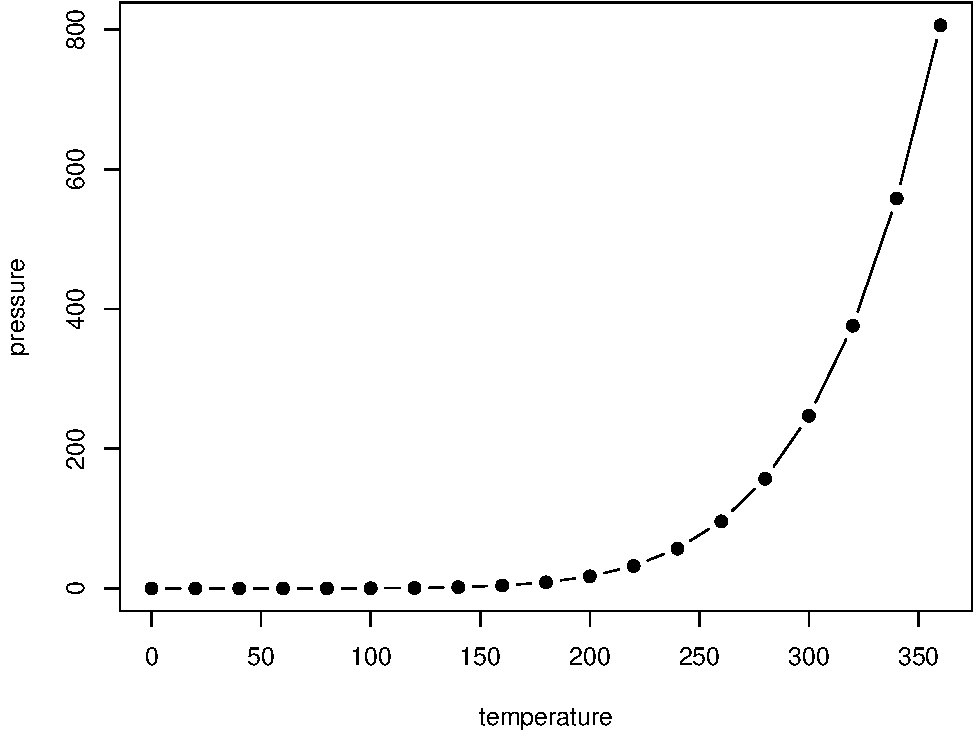
\includegraphics[width=0.8\linewidth]{_main_files/figure-latex/nice-fig-1} 

}

\caption{Here is a nice figure!}\label{fig:nice-fig}
\end{figure}

Don't miss Table \ref{tab:nice-tab}.

\begin{Shaded}
\begin{Highlighting}[]
\NormalTok{knitr}\SpecialCharTok{::}\FunctionTok{kable}\NormalTok{(}
  \FunctionTok{head}\NormalTok{(pressure, }\DecValTok{10}\NormalTok{), }\AttributeTok{caption =} \StringTok{\textquotesingle{}Here is a nice table!\textquotesingle{}}\NormalTok{,}
  \AttributeTok{booktabs =} \ConstantTok{TRUE}
\NormalTok{)}
\end{Highlighting}
\end{Shaded}

\begin{table}

\caption{\label{tab:nice-tab}Here is a nice table!}
\centering
\begin{tabular}[t]{rr}
\toprule
temperature & pressure\\
\midrule
0 & 0.0002\\
20 & 0.0012\\
40 & 0.0060\\
60 & 0.0300\\
80 & 0.0900\\
\addlinespace
100 & 0.2700\\
120 & 0.7500\\
140 & 1.8500\\
160 & 4.2000\\
180 & 8.8000\\
\bottomrule
\end{tabular}
\end{table}

\newpage

\chapter{Parts}\label{parts}

You can add parts to organize one or more book chapters together. Parts can be inserted at the top of an .Rmd file, before the first-level chapter heading in that same file.

Add a numbered part: \texttt{\#\ (PART)\ Act\ one\ \{-\}} (followed by \texttt{\#\ A\ chapter})

Add an unnumbered part: \texttt{\#\ (PART\textbackslash{}*)\ Act\ one\ \{-\}} (followed by \texttt{\#\ A\ chapter})

Add an appendix as a special kind of un-numbered part: \texttt{\#\ (APPENDIX)\ Other\ stuff\ \{-\}} (followed by \texttt{\#\ A\ chapter}). Chapters in an appendix are prepended with letters instead of numbers.

\newpage

\chapter{Footnotes and citations}\label{footnotes-and-citations}

\section{Footnotes}\label{footnotes}

Footnotes are put inside the square brackets after a caret \texttt{\^{}{[}{]}}. Like this one \footnote{This is a footnote.}.

\section{Citations}\label{citations}

Reference items in your bibliography file(s) using \texttt{@key}.

For example, we are using the \textbf{bookdown} package \autocite{R-bookdown} (check out the last code chunk in index.Rmd to see how this citation key was added) in this sample book, which was built on top of R Markdown and \textbf{knitr} \autocite{xie2015} (this citation was added manually in an external file book.bib).
Note that the \texttt{.bib} files need to be listed in the index.Rmd with the YAML \texttt{bibliography} key.

The RStudio Visual Markdown Editor can also make it easier to insert citations: \url{https://rstudio.github.io/visual-markdown-editing/\#/citations}

\newpage

\chapter{Blocks}\label{blocks}

\section{Equations}\label{equations}

Here is an equation.

\begin{equation}
  f\left(k\right) = \binom{n}{k} p^k\left(1-p\right)^{n-k}
  \label{eq:binom}
\end{equation}

You may refer to using \texttt{\textbackslash{}@ref(eq:binom)}, like see Equation \eqref{eq:binom}.

\section{Theorems and proofs}\label{theorems-and-proofs}

Labeled theorems can be referenced in text using \texttt{\textbackslash{}@ref(thm:tri)}, for example, check out this smart theorem \ref{proof:tri}.

\begin{proof}[]
For a right triangle, if \(c\) denotes the \emph{length} of the hypotenuse
and \(a\) and \(b\) denote the lengths of the \textbf{other} two sides, we have
\[a^2 + b^2 = c^2\]
\end{proof}

Read more here \url{https://bookdown.org/yihui/bookdown/markdown-extensions-by-bookdown.html}.

\section{Callout blocks}\label{callout-blocks}

The R Markdown Cookbook provides more help on how to use custom blocks to design your own callouts: \url{https://bookdown.org/yihui/rmarkdown-cookbook/custom-blocks.html}

\newpage

\chapter{Sharing your book}\label{sharing-your-book}

\section{Publishing}\label{publishing}

HTML books can be published online, see: \url{https://bookdown.org/yihui/bookdown/publishing.html}

\section{404 pages}\label{pages}

By default, users will be directed to a 404 page if they try to access a webpage that cannot be found. If you'd like to customize your 404 page instead of using the default, you may add either a \texttt{\_404.Rmd} or \texttt{\_404.md} file to your project root and use code and/or Markdown syntax.

\section{Metadata for sharing}\label{metadata-for-sharing}

Bookdown HTML books will provide HTML metadata for social sharing on platforms like Twitter, Facebook, and LinkedIn, using information you provide in the \texttt{index.Rmd} YAML. To setup, set the \texttt{url} for your book and the path to your \texttt{cover-image} file. Your book's \texttt{title} and \texttt{description} are also used.

This \texttt{gitbook} uses the same social sharing data across all chapters in your book- all links shared will look the same.

Specify your book's source repository on GitHub using the \texttt{edit} key under the configuration options in the \texttt{\_output.yml} file, which allows users to suggest an edit by linking to a chapter's source file.

Read more about the features of this output format here:

\url{https://pkgs.rstudio.com/bookdown/reference/gitbook.html}

Or use:

\begin{Shaded}
\begin{Highlighting}[]
\NormalTok{?bookdown}\SpecialCharTok{::}\NormalTok{gitbook}
\end{Highlighting}
\end{Shaded}

\newpage

% Back matter
\backmatter

% Bibliography
\printbibliography[heading=bibintoc,title=References]

% Vita Auctoris
\cleardoublepage
\phantomsection
\addcontentsline{toc}{chapter}{Vita Auctoris}
\chapter*{Vita Auctoris}
\begin{doublespace}
Your Name was born in {[}Place{]}, {[}Date{]}. He/She attended {[}University Name{]} and received a B.S. in {[}Field{]} in {[}Year{]}. He/She then pursued graduate studies at {[}University Name{]}, earning an M.S. in {[}Field{]} in {[}Year{]}. During his/her doctoral studies at {[}University Name{]}, he/she {[}brief description of research or notable achievements{]}. He/She has published {[}number{]} papers in {[}field{]} journals and presented his/her work at {[}number{]} international conferences. Upon completion of his/her Ph.D., he/she plans to {[}future plans or career goals{]}.
\end{doublespace}

\end{document}
